\documentclass{article}
\usepackage{graphicx}
\usepackage{hyperref}
\usepackage{svg}
\usepackage{pdfpages}
\usepackage{tikz}

%Here is an example of a LaTeX script that you can use as a starting point for creating the conference handbook for your Taiwan-Somaliland Medical Conference in August 2023:

%```latex by chatGPT

%% x
%\title{2023 COLLABORATING FOR BETTER HEALTH:
%A MULTI-SPECIALTY CONFERENCE}
%\date{13-14 August 2023}

\begin{document}

%\begin{center} % to remove Fig.
%\end{center}

\begin{titlepage}
%    \centering

%\begin{center}
\hspace*{-0.7cm}%
\begin{tikzpicture} % tikzfigure
%\begin{minipage}[b]{1\linewidth}

\includesvg[height=3.0cm, distort=false]{Flag_of_the_Republic_of_China.svg}
\hspace{1.4cm}
%\includesvg[width=0.17\linewidth]{TMM_logo.svg}
%\hspace{3cm}
\includesvg[height=3.0cm, distort=false]{Flag_of_Somaliland.svg}
%\captionof{Figure}{xx}
%\end{minipage}
\end{tikzpicture}
    \vspace{4cm}
    
\centering
    {\Huge\bfseries % Taiwan---Somaliland \\
    2023 COLLABORATING FOR BETTER HEALTH:
A MULTI-SPECIALTY CONFERENCE\\
    Handbook\par}
    \vspace{1.5cm}
    %\hspace{4cm} 
    {\Large 13-14 August 2023\par}

%\end{center}

\vspace{2.5cm}

\includesvg[height=4.0cm, distort=false]{TMM_logo.svg}


\end{titlepage}


%\maketitle

\clearpage

\section*{Overview}
In August of 2023, Taiwan and Somaliland will host a medical conference. Medical professionals from around the country gather at this conference to exchange ideas and discuss recent advancements. Hemodialysis, live-donor organ transplants, forensics, otolaryngology, oral and maxillofacial surgery, non-communicable illnesses, the Taiwanese experience with HBV/HCV, and the present situation in Somaliland are just a few of the topics that will be discussed during the conference. We anticipate that by disseminating this knowledge to medical professionals in many public hospitals and private sectors in major cities across Somaliland, we may encourage sharing knowledge and best practices amongst them and eventually enhance patient care.


\section*{Conference Schedule}
The conference will take place over two half days in the morning on August 13 and August 14.

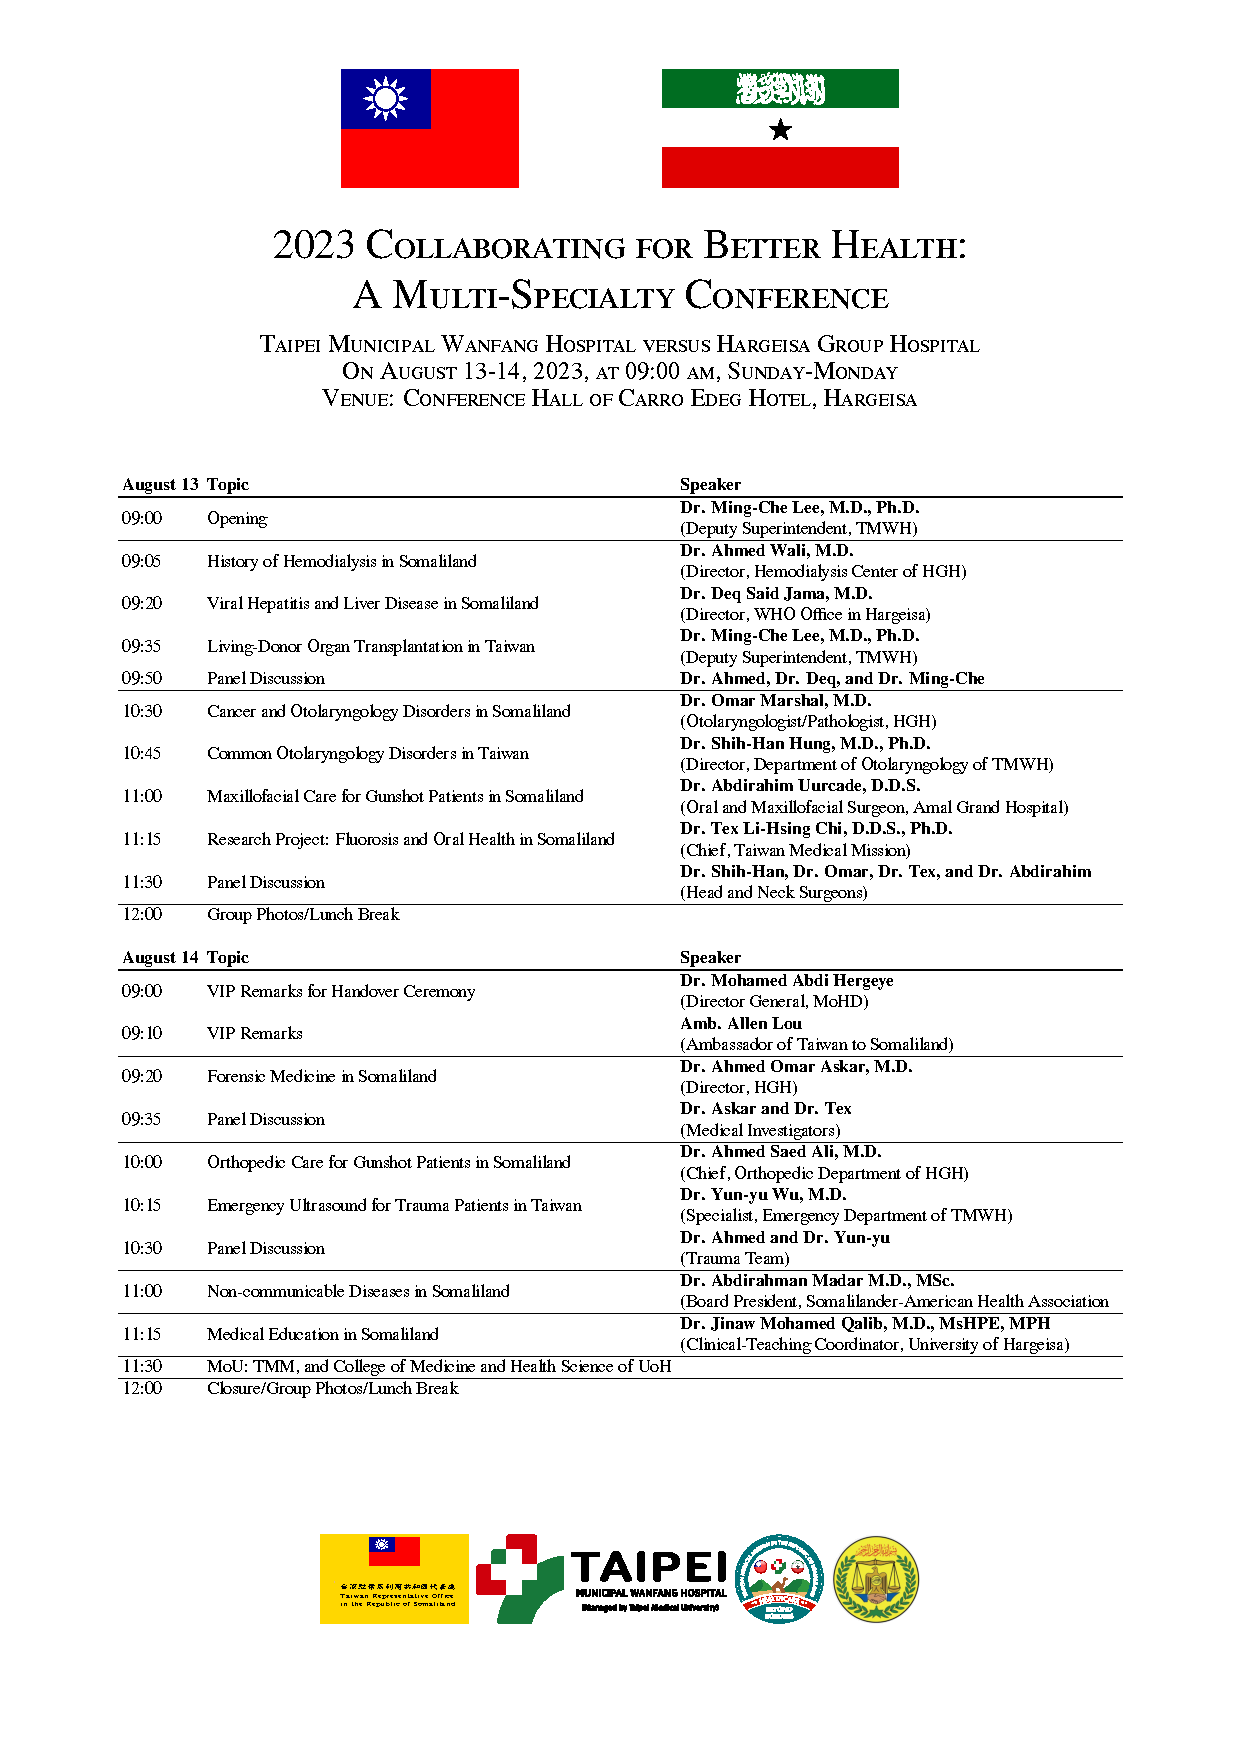
\includepdf[page={1}]{TMM_SLN_tikzposter_2023Aug__portrait_agenda___TMM_Conference.pdf}
%\section{agenda}

%%%%%%%
%\captionsetup{labelformat=empty} % 
\begin{center} % to remove Fig.
    
\begin{tikzfigure}[]
%\begin{minipage}[b]{1\linewidth}

%Taiwan\\
%\vspace{5cm}
\includesvg[height=2.0cm, distort=false]{Flag_of_the_Republic_of_China.svg}
\hspace{2cm}
%\includesvg[width=0.17\linewidth]{TMM_logo.svg}
%\hspace{3cm}
\includesvg[height=2.0cm, distort=false]{Flag_of_Somaliland.svg}
%\captionof{Figure}{xx}
%\end{minipage}
\end{tikzfigure}

\end{center}


%%% title; font size and baseline offset (line space)
\fontsize{20}{24} \sc
2023 Collaborating for Better Health: \\
A Multi-Specialty Conference \\
%on Taiwan and Somaliland
 \par
\vspace{0.3cm}
% FOR MINISTRY OF HEALTH DEVELOPMENT

\fontsize{12}{13} \sc
Taipei Municipal Wanfang Hospital versus Hargeisa Group Hospital\\
On August 13-14, 2023, at 09:00 am, Sunday-Monday \\
Venue: Conference Hall of Carro Edeg Hotel, Hargeisa
%Exhibition Hall of the Hargeisa Group Hospital
% no more Jees Hotel
\par
%\vspace{0.2cm}
%%%%%%%%%%%%




% agenda
%\begin{columns}

%\column{0.7}
%\block{Agenda}{

\begin{center}
    
%\begin{minipage}{0.9\linewidth}

% Please add the following required packages to your document preamble:
% \usepackage{graphicx}
\begin{table}[h]
\centering
\resizebox{1.00\textwidth}{!}{%
\begin{tabular}{llll}
%%%% day 1
\textbf{August 13} & \textbf{Topic}       & \textbf{Speaker}                                                                            & \textbf{} \\ \hline  \hline

09:00         & Opening                 & \begin{tabular}[c]{@{}l@{}} \textbf{Dr. Ming-Che Lee, M.D., Ph.D.}\\ (Deputy Superintendent, TMWH)\end{tabular}    
&           \\ \hline

09:05         & Hemodialysis and Renal Failure in Somaliland                 & \begin{tabular}[c]{@{}l@{}} \textbf{Dr. Ahmed Wali, M.D.}\\ (Director, Hemodialysis Center of HGH)\end{tabular}    
&           \\

09:20         & Viral Hepatitis and Liver Disease in Somaliland                 & \begin{tabular}[c]{@{}l@{}} \textbf{Dr. Deq Said Jama, M.D.}\\ (Director, WHO Office in Hargeisa)\end{tabular}    
&           \\

09:35         & Living-Donor Organ Transplantation in Taiwan                 & \begin{tabular}[c]{@{}l@{}} \textbf{Dr. Ming-Che Lee, M.D., Ph.D.}\\ (Deputy Superintendent, TMWH)\end{tabular}    
&           \\

% MoU of Hemodialysis Center---Transplant Team
09:50         & Panel Discussion           & \begin{tabular}[c]{@{}l@{}} \textbf{Dr. Ahmed, Dr. Deq, and Dr. Ming-Che}\\ 
\end{tabular}    
&           \\ \hline



%%%


10:30         & Common Otolaryngology Disorders in Somaliland   
& \begin{tabular}[c]{@{}l@{}} \textbf{Dr. Hersi Dahir Madar, M.D.} \\(Otolaryngologist, HGH) \end{tabular}                                                &           \\

10:45         & Common Otolaryngology Disorders in Taiwan   & \begin{tabular}[c]{@{}l@{}} \textbf{Dr. Shih-Han Hung, M.D., Ph.D.} \\(Director, Department of Otolaryngology of TMWH) \end{tabular}                                                &           \\
%%%

11:00         & Maxillofacial Care for Gunshot Patients in Somaliland  & \begin{tabular}[c]{@{}l@{}} \textbf{Dr. Abdirahim Uurcade, D.D.S.} \\(Oral and Maxillofacial Surgeon, Amal Grand Hospital) \end{tabular}                                                          &           \\

11:15         & Oral Health and Khat-leaf Use in Somaliland & \begin{tabular}[c]{@{}l@{}} \textbf{Dr. Tex Li-Hsing Chi, D.D.S., Ph.D.} \\(Chief, Taiwan Medical Mission) \end{tabular}                                                          &           \\



11:30         & Panel Discussion  & \begin{tabular}[c]{@{}l@{}} \textbf{Dr. Shih-Han, Dr. Omar, Dr. Tex, and Dr. Abdirahim}\\ (Head and Neck Surgeons) \end{tabular} &           \\  \hline

%11:20         & Emergency Ultrasound  & \begin{tabular}[c]{@{}l@{}} \textbf{Dr. Yun-yu Wu, M.D.} \\ 
%(Department of Emergency, TMWH)  \end{tabular}                                                                                     &           \\

%10:20         & Remark for the Project  & \begin{tabular}[c]{@{}l@{}} \textbf{ Mr. Allen Lou }\\ (Ambassador of Taiwan in Somaliland)\end{tabular}  &           \\

12:00         & Group Photos/Lunch Break            &                                                                                             &           \\
%12:35         & Refreshment &                                                                                             &   \\ 


%%%%%%%%%%%%%%%%%%%%%%%%% day 2
\\
\textbf{August 14} & \textbf{Topic}       & \textbf{Speaker}                                                                            & \textbf{} \\  \hline  \hline

09:00         & VIP Remarks for Handover Ceremony                 & \begin{tabular}[c]{@{}l@{}} \textbf{Dr. Mohamed Abdi Hergeye}\\ (Director General, MoHD)\end{tabular} &           \\  

09:10         &   & \begin{tabular}[c]{@{}l@{}} \textbf{Amb. Allen Lou }\\ (Ambassador of Taiwan to Somaliland)\end{tabular}  &           \\ \hline

09:20         & Forensic Medicine in Somaliland   & \begin{tabular}[c]{@{}l@{}} \textbf{Dr. Ahmed Omar Askar, M.D.} \\(Director, HGH) \end{tabular}                                                &           \\

%09:20         & Forensic Medicine in Taiwan   & \begin{tabular}[c]{@{}l@{}} \textbf{Dr. Tex Li-Hsing Chi, D.D.S., Ph.D.} \\(Chief, Taiwan Medical Mission)  \end{tabular}                                                &           \\
%%% Taiwan Medical Mission,對於HGH的幫助等效益

09:35         & Panel Discussion  & \begin{tabular}[c]{@{}l@{}} \textbf{Dr. Askar and Dr. Tex}\\ (Medical Investigators) \end{tabular} &           \\  \hline

%%% 台灣捐贈的骨科設備,對於索國骨科醫師的幫助等效益
10:00         & Orthopedic Care for Gunshot Patients in Somaliland   & \begin{tabular}[c]{@{}l@{}} \textbf{Dr. Ahmed Saed Ali, M.D.} \\(Chief, Orthopedic Department of HGH) \end{tabular}                                                          &           \\

10:15         & Emergency Ultrasound for Trauma Patients in Taiwan  & \begin{tabular}[c]{@{}l@{}} \textbf{Dr. Yun-yu Wu, M.D.} \\ 
(Specialist, Emergency Department of TMWH)  \end{tabular}                                                                                     &           \\
10:30         & Panel Discussion  & \begin{tabular}[c]{@{}l@{}} \textbf{Dr. Ahmed and Dr. Yun-yu}\\ (Trauma Team) \end{tabular} &           \\  \hline

%%
11:00         & Non-communicable Diseases in Somaliland  &  \begin{tabular}[c]{@{}l@{}} \textbf{Dr. Abdirahman Madar
M.D., MSc.} \\ (Board President, Somalilander-American Health Association \end{tabular}  &           \\ \hline

%11:20         & Introduction of Viral Hepatitis in Somaliland  &  \begin{tabular}[c]{@{}l@{}} \textbf{Dr. Abdulkani Yusuf, M.D.} \\ (Director of City Hospital) \end{tabular}                                                                                &           \\
%10:20         & Remark for the Project  & \begin{tabular}[c]{@{}l@{}} \textbf{ Mr. Allen Lou }\\ (Ambassador of Taiwan in Somaliland)\end{tabular}  &           \\

% Dr. Jinaw Mohamed Qalib, M.D., MsHPE, MPH (Clinical-Teaching Coordinator, University of Hargiesa)
11:15         & Medical Education in Somaliland  &  \begin{tabular}[c]{@{}l@{}} \textbf{Dr. Jinaw Mohamed Qalib, M.D., MsHPE, MPH} \\ (Clinical-Teaching Coordinator, University of Hargeisa) \end{tabular}  &           \\ \hline

11:30         & MoU: TMM, and College of Medicine and Health Science of UoH            &                                                                                             &           \\ \hline
12:00         & Closure/Group Photos/Lunch Break &                                                                                             &   \\  


\end{tabular}%
} % end of resizebox


\end{table}


%\end{minipage}

\end{center}



%%%%%%%%%%%

%%% footer
%\block{}{
%\node [above right,
%       outer sep=0pt,
%       minimum width=\paperwidth-2*\pgflinewidth,
%       minimum height=7cm,
%       align=center,font=\Huge,
%       draw,fill=green!30,
%       ultra thick] at ([shift={(0.5*\pgflinewidth,0.5*\pgflinewidth)}]bottomleft) 
%       {

\begin{tikzfigure}[]
%\includesvg[height=40.0cm, distort=false]{ortho_ward_Tex_Josh.svg}

%\includesvg[height=2.5cm, distort=false]{TRO_Somaliland.svg} \hspace{2cm}
%\includesvg[height=2.5cm, distort=false]{MoHD_Somaliland.svg}

%\hspace{1cm} % https://mohd.govsomaliland.org/
%\includegraphics{TMWH_scope.pdf}


%*** using zong Kai Chinese font by \ZongKai{}, and adjust image size \scalebox{h}[v]{}
% image and character: \resizebox{2.7cm}{1.5cm}{}
\ZongKai{\fontsize{3.3}{6}\selectfont \scalebox{1.3}[1.0]{\includesvg[height=1.5cm, distort=false]{TRO_Somaliland.svg}}}
\includesvg[height=1.5cm]{TMWH_logo_TAIPEI_vector.svg}
%\includesvg[height=25.0cm, distort=false]{TRO_Somaliland_font_ZongKai.svg.svg}\hspace{1cm} % TRO logo with ZongKai font in path
\includesvg[height=1.5cm, distort=false]{TMM_logo.svg}
%{2023TMM_officePlate_pink.svg}
\includesvg[height=1.5cm, distort=false]{Hargeisa_Group_Hospital_logo.svg}
\includesvg[height=1.5cm, distort=false]{MoHD_Somaliland.svg} % 2020
%\includegraphics[height=12.0cm, distort=false]{2023TMM_officePlate_ai.pdf}

%%% *********
% ?? add logo of military and social welfare ??

\end{tikzfigure}



%}; % end of node

%} % end of block


%\subsection*{August 13}
%\begin{itemize}
%    \item 9:00 AM - Opening remarks
%    \item 9:30 AM - Keynote speaker
%    \item 10:30 AM - Break
%    \item 11:00 AM - Session 1
%    \item 12:00 PM - Lunch
%\end{itemize}

%\subsection*{August 14}
%\begin{itemize}
%    \item 9:00 AM - Session 2
%    \item 10:00 AM - Break
%    \item 10:30 AM - Session 3
%    \item 11:30 AM - Closing remarks
%    \item 12:00 PM - Lunch
%\end{itemize}

\section*{Speaker Biographies}
% Add speaker biographies or CVs here

\section*{Abstracts of Presentations}
% Add abstracts of presentations here

% Tex Chi
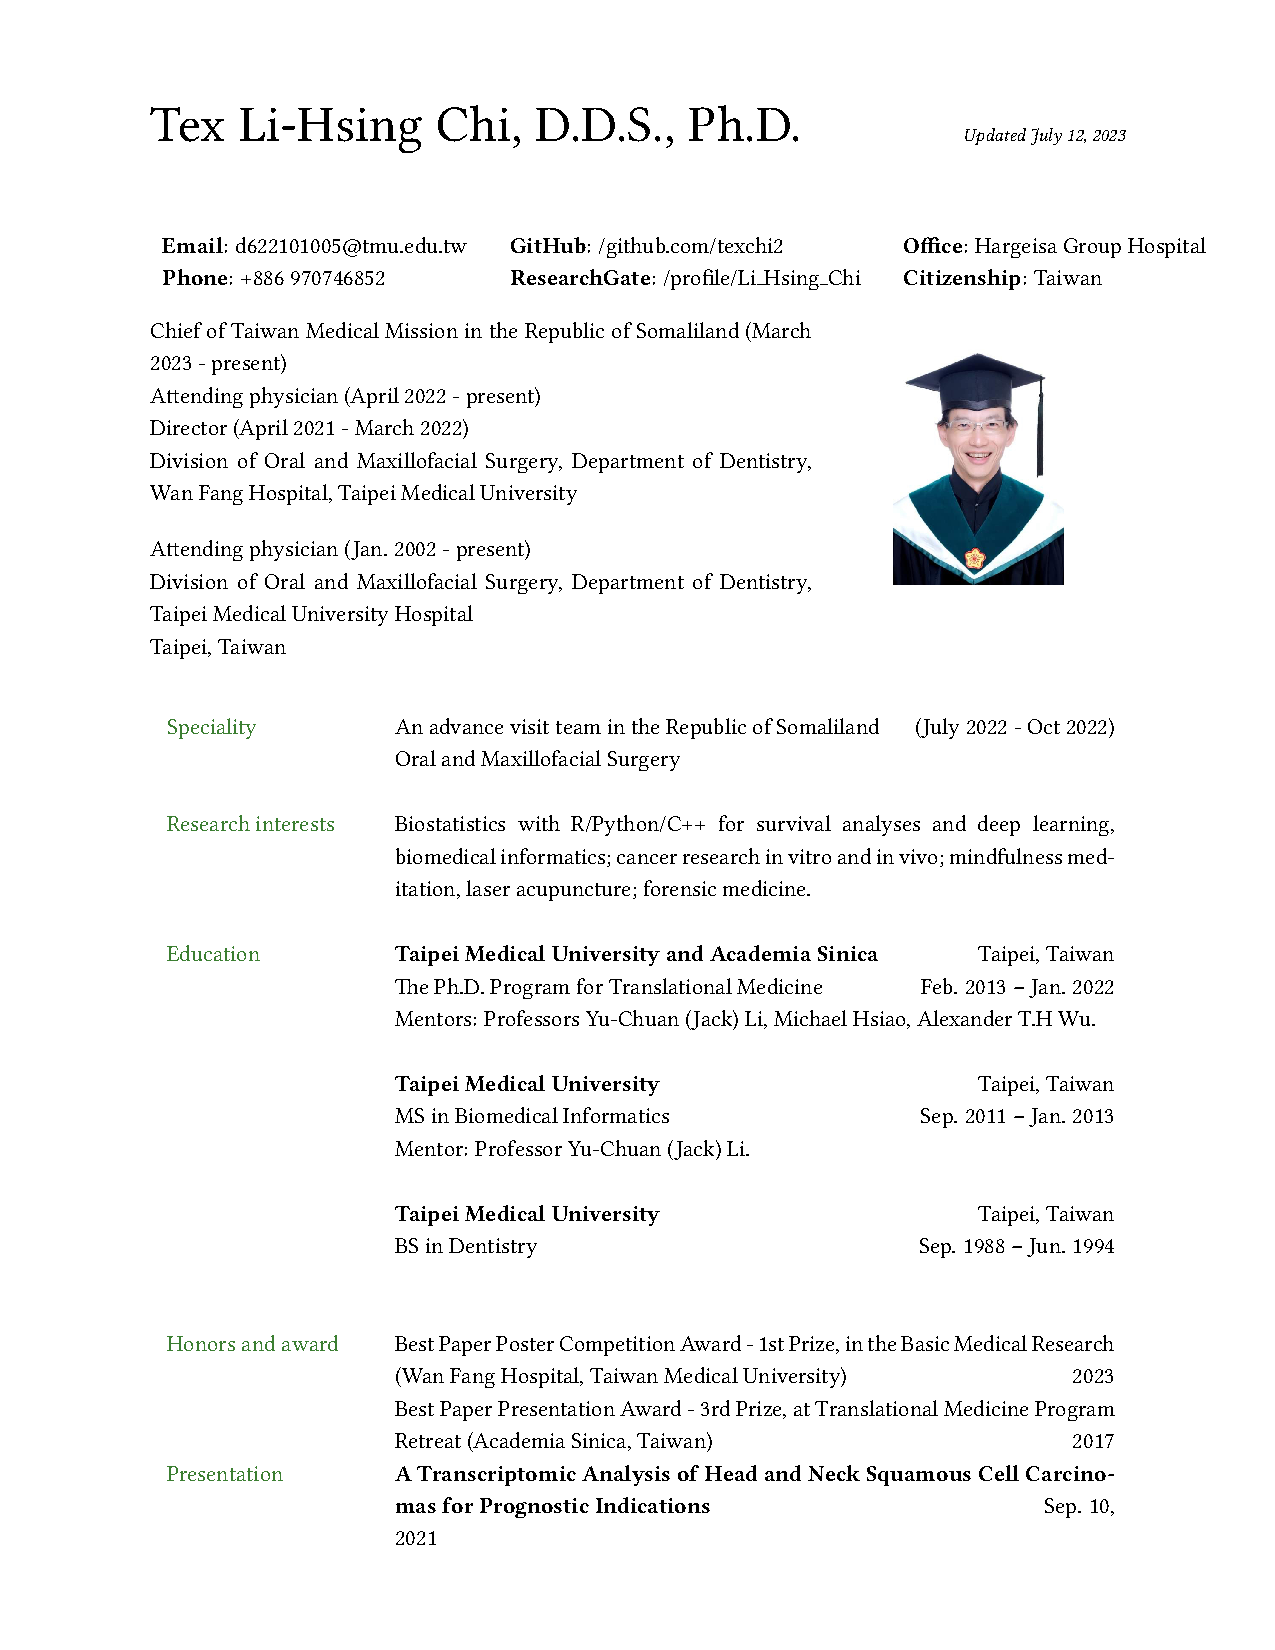
\includepdf[pages={1}]{AcademicCV_Li_Hsing_Chi2023.pdf}

\includepdf[pages={1,2}]{HGH_research_proposal_fluorosis_DrMukhtar_DrFadomu.pdf}


\end{document}
```

